\chapter{Vícerozměrná regresní analýza - odhad}

\section{Úvod}

\subsection{Dvourozměrný regresní model}

Dvourozměrný regresní model má tvar
\begin{equation}
y = \beta_0 + \beta_1 x_1 + \beta_2 x_2 + u,
\end{equation}
kde $\beta_0$ je průsečík regresního modelu a $\beta_1$ resp. $\beta_2$ vyjadřuje sklon vzhledem k $x_1$ resp. $x_2$ za předpokladu fixace ostatních faktorů.

Podobně jako v případě jednoduchého regresního modelu platí
\begin{equation}
E[u|x_1, x_2] = 0,
\end{equation}
tj. pro libovolné hodnoty $x_1$ a $x_2$ je průměrný vliv faktorů zachycený chybou $u$ roven 0. Vzhledem k tomu, že je v 
modelu zahrnut průsečík $\beta_0$, nejedná se o předpoklad, ale o důsledek specifikace modelu.

\subsection{Vícerozměrný regresní model}

Vícerozměrný regresní model má tvar
\begin{equation}
y = \beta_0 + \beta_1 x_1 + \beta_2 x_2 + ... + \beta_k x_k + u
\end{equation}
a opět platí
\begin{equation}
E[u|x_1, x_2, ..., x_k] = 0.
\end{equation}

\section{Metoda nejmenších čtverců}

\subsection{OLS odhady}

Uvažujme odhad dvourozměrného regresního modelu
\begin{equation}
\hat{y} = \hat{\beta}_0 + \hat{\beta}_1 x_1 + \hat{\beta}_2 x_2.
\end{equation}
Odhady $\hat{\beta}_0$, $\hat{\beta}_1$ a $\hat{\beta}_2$ jsou zvoleny tak, aby minimalizovaly
\begin{equation}
\sum_{i = 1}^n (y_i - \hat{\beta}_0 - \hat{\beta}_1 x_{i1} - \hat{\beta}_2 x_{i2})^2.
\end{equation}
Analogicky v případě odhadu $k$-rozměrného regresního modelu
\begin{equation}
\hat{y} = \hat{\beta}_0 + \hat{\beta}_1 x_1 + \hat{\beta}_2 x_2 + ... + \hat{\beta}_k x_k
\end{equation}
jsou $\hat{\beta}_0$ až $\hat{\beta}_k$ zvoleny tak, aby minimalizovaly
\begin{equation}
\sum_{i = 1}^n (y_i - \hat{\beta}_0 - \hat{\beta}_1 x_{i1} - \hat{\beta}_2 x_{i2} - ... - \hat{\beta}_k x_{ik})^2.
\end{equation}

\subsection{Interpretace OLS regresní rovnice}

Odhady $\hat{\beta}_1$ a $\hat{\beta}_2$ dvourozměrného regresního modelu lze vzhledem vysvětlované veličině $y$ interpretovat jako 
\begin{equation}
\Delta \hat{y} = \hat{\beta}_1 \Delta x_1 + \hat{\beta}_2 \Delta x_2.
\end{equation}
Analogicky odhady $k$-rozměrného regresního modelu lze interpretovat jako
\begin{equation}
\Delta \hat{y} = \hat{\beta}_1 \Delta x_1 + \hat{\beta}_2 \Delta x_2 + ... + \hat{\beta}_k \Delta x_k.
\end{equation}

\subsection{Predikované hodnoty a rezidua}

Hodnoty predikované odhadnutým $k$-rozměrným regresním modelem  a odpovídající rezidua jsou definovány jako
\begin{equation}
\hat{y}_i = \hat{\beta}_0 + \hat{\beta}_1 x_{i1} + \hat{\beta}_2 x_{i2} + ... + \hat{\beta}_k x_{ik}
\end{equation}
a
\begin{equation}
\hat{u}_i = y_i - \hat{y}_i.
\end{equation}
Predikované hodnoty a rezidua mají některé důležité vlastnosti, které jsou analogií jejich vlastností v 
rámci jednoduchého regresního modelu.
\begin{itemize}
\item Protože $E[\hat{u}] = 0$, platí $\bar{y} = \bar{\hat{y}}$.
\item Protože $cov[x_j,\hat{u}] = 0$ pro libovolný pár vysvětlující veličiny $x_j$ a $\hat{u}$, platí 
$cov[\hat{y}, \hat{u}] = 0$.
\item Bod $\bar{x}_1, \bar{x}_2, ..., \bar{x}_k, \bar{y}$ leží vždy na OLS regresní přímce, tj. $\bar{y} = 
\hat{\beta}_0 + \hat{\beta}_1 \bar{x}_1 + \hat{\beta}_2 \bar{x}_2 + ... + \hat{\beta}_k \bar{x}_k$.
\end{itemize}

\subsection{Odhad sklonu ve vícerozměrném regresním modelu}

Uvažujme dvourozměrný regresní model $y = \beta_0 + \beta_1 x_1 + \beta_2 x_2 + u$. Regresní parametr $\beta_1$ lze odhadnout na základě rovnice
\begin{equation}
\hat{\beta}_1 = \frac{\sum_{i = 1}^n \hat{r}_{i1}y_i}{\sum_{i = 1}^n \hat{r}_{i1}^2},
\end{equation}
kde $\hat{r}_{i1}$ představuje rezidua z odhadu jednoduchého regresního modelu $x_1 = \beta_0^* + \beta_1^* x_2 + u$. 
Výše uvedená rovnice nám pak říká, že stačí aplikovat regresi $y$ na $\hat{r}_1$, abychom získali odhad 
$\hat{\beta}_1$ původního regresního modelu\footnote{Protože střední hodnota reziduí $\hat{r}_{i1}$ je rovna 
nule, je $\hat{\beta}_1$ standardním odhadem sklonu jednoduchého regresního modelu.}. Protože $\hat{r}_{i1}$ 
představuje tu část $x_{i1}$, která je nekorelovaná s $x_{i2}$, lze $\hat{r}_{i1}$ chápat jako $x_{i1}$ po té, 
co byl odstraněn vliv $x_{i2}$. Jinými slovy $\hat{\beta}_1$ v rovnici $\hat{y} = \hat{\beta}_0 + \hat{\beta}_1 x_1 + 
\hat{\beta}_2 x_2$ vyjadřuje změnu $y$ při zvýšení $x_1$ o jednu jednotku a za předpokladu fixního $x_2$.

V případě $k$ rozměrného regresního modelu lze $\beta_1$ stále odhadnout pomocí (3.13), nicméně tentokrát 
budou rezidua $\hat{r}_{i1}$ výstupem regrese $x_1$ na $x_2, x_3, ..., x_k$. $\hat{\beta}_1$ tak vyjadřuje dopad 
změny $x_1$ na $y$ za předpokladu fixace $x_2, x_3, ..., x_k$.

\subsection{Porovnání odhadů jednoduchého a vícerozměrného regresního modelu}

Uvažujme odhad jednoduchého regresního modelu $\tilde{y} = \tilde{\beta}_0 + \tilde{\beta}_1 x_1$ a 
vícerozměrného modelu $\hat{y} = \hat{\beta}_0 + \hat{\beta}_0 x_1 + \hat{\beta}_1 x_2$. Vztah mezi 
$\tilde{\beta}_1$ a $\hat{\beta}_1$ je dán
\begin{equation}
\tilde{\beta}_1 = \hat{\beta}_1 + \hat{\beta}_2 \tilde{\delta}_1,
\end{equation}
kde $\tilde{\delta}_1$ je sklon jednoduchého regresního modelu $x_2 = \tilde{\delta}_0 + \tilde{\delta}_1 x_1 + u$. Z (3.14) také 
vyplývá, že $\tilde{\beta}_1 = \hat{\beta}_1$, jestliže
\begin{itemize}
\item parciální efekt $x_2$ na $\hat{y}$ je nulový, tj. $\hat{\beta}_2 = 0$ nebo
\item $x_1$ a $x_2$ jsou v rámci vzorku, na základě kterého odhadujeme regresní model, nekorelované, tj. 
$\tilde{\delta}_1 = 0$.
\end{itemize}

V případě $k$ nezávislých veličin dá jednoduchý regresní model $y$ na $x_1$ a vícerozměrný regresní model 
$y$ na $x_1, x_2, ..., x_k$ stejný odhad sklonu vzhledem k $x_1$ pouze tehdy, jestliže (1) odhady sklonu vzhledem k 
$x_2$ až $x_k$ jsou nulové nebo (2) $x_1$ je nekorelované s $x_2$ až $x_k$.

\subsection{Míra shody}

Stejně jako v případě jednoduchého regresního modelu jsou 
celkový součet čtverců SST, vysvětlený součet čtverců SSE a reziduální součet čtverců SSR definovány jako
\begin{equation}
SST \equiv \sum_{i = 1}^n(y_i - \bar{y})^2,
\end{equation}
\begin{equation}
SSE \equiv \sum_{i = 1}^n (\hat{y}_i - \bar{y})^2
\end{equation}
a
\begin{equation}
SSR \equiv \sum_{i = 1}^n \hat{u}_i^2.
\end{equation}
Dále opět platí
\begin{equation}
SST = SSE + SSR.
\end{equation}
Ukazatel míry shody $R^2$ je identicky definován jako
\begin{equation}
R^2 \equiv \frac{SSE}{SST} = 1 - \frac{SSR}{SST},
\end{equation}
což lze též vyjádřit ve tvaru
\begin{equation}
R^2 = \frac{\left(\sum_{i = 1}^n (y_i - \bar{y})(\hat{y}_i - \bar{\hat{y}})\right)^2}{\left(\sum_{i = 1}^n(y_i - 
\bar{y})^2\right)\left(\sum_{i = 1}^n (\bar{y}_i - \bar{\hat{y}})^2\right)}.
\end{equation}
Bohužel $R^2$ téměř vždy vzroste, pokud do regresního modelu přidáme další vysvětlující veličinu. To je 
dáno tím, že při rozšíření modelu o další vysvětlující veličinu SSR nikdy nevzroste (naopak typicky klesne), zatímco SST 
zůstává  stejné. Protože $R^2$ postrádá penalizaci za počet vysvětlujících proměnných zahrnutých v regresním 
modelu, nelze ho použít při rozhodování o tom, zda-li má být určitá veličina do něj přidána či nikoliv.

\subsection{Regresní model bez průsečíku}

Vícerozměrný regresní model bez průsečíku má podobu
\begin{equation}
\tilde{y} = \tilde{\beta}_1 x_1 + \tilde{\beta}_2 x_2 + ... + \tilde{\beta}_k x_k.
\end{equation}
Vlastnosti OLS, které jsme výše zmiňovali, nejsou pro vícerozměrný regresní model bez průsečíku platné. Konkrétně průměr 
reziduí $\hat{u}_i$ není roven nule a $R^2$ může být záporné\footnote{Aby se vyhnuli tomuto problému, 
preferují někteří ekonometři definovat $R^2$ jako druhou mocninu korelačního koeficientu mezi aktuálními a 
predikovanými hodnotami $y_i$.}. Dále, je-li $\beta_0$ populačního regresního modelu ve skutečnosti různé od 
nuly, jsou odhady sklonů vůči jednotlivým vysvětlujícím proměnným zkreslené.

\section{Očekávaná hodnota OLS odhadů}

Podobně jako v případě jednoduchého regresního modelu také u vícerozměrného modelu zahájíme tuto kapitolu 
výčtem předpokladů, na kterých staví metodologie OLS odhadů.

\begin{assumption}[MLR.1 - lineární model]
Populační regresní model lze vyjádřit ve tvaru
\begin{equation}
y = \beta_0 + \beta_1 x_1 + \beta_2 x_2 + ... + \beta_k x_k + u,
\end{equation}
kde $\beta_0, \beta_1, ..., \beta_k$ jsou neznámé parametry modelu a $u$ je nepozorovatelná náhodná chyba.

\raggedleft{$\clubsuit$}
\end{assumption}

\begin{assumption}[MRL.2 - náhodný výběr]
Máme k dispozici náhodný výběr velikosti $n$, $\{(x_{i1}, x_{i2}, ..., x_{i3}, y_i): i = 1, 2, ..., n\}$, který 
sleduje populační model definovaný v předpokladu MRL.1.

\raggedleft{$\clubsuit$}
\end{assumption}

\begin{assumption}[MLR.3 - neexistence perfektní kolinearity]
V populaci (a tím pádem také v náhodném výběru) není žádná z vysvětlujících veličin konstantní a 
žádná vysvětlující proměnná není lineární kombinací zbývajících. V opačném případě trpí model tzv. 
perfektní kolinearitou\footnote{Jednotlivé vysvětlující proměnné mohou být korelovány; nesmějí však být 
dokonale korelovány. V případě dokonalé korelace nelze tvrdit, že měníme jednu z vysvětlujících veličin, 
zatímco ostatní jsou fixní.}.

\raggedleft{$\clubsuit$}
\end{assumption}

Problém perfetní multikolinearity může být na první pohled skrytý. Jako příklad uvažujme model, ve 
kterém zkoumáme souvislost mezi výdaji státu na vzdělání a obranu a hrubým domácím produktem. Trochu 
zjednodušeně předpokládejme, že se jedná o jediné výdaje státu. Správně definovaný regresní model má tvar
\begin{equation}
gdp = \beta_0 + \beta_1 expense_{tot} + \beta_2 expense_{educ} + u
\end{equation}
zatímco regresní model ve tvaru
\begin{equation}
gdp = \beta_0 + \beta_1 expense_{tot} + \beta_2 expense_{educ} + \beta_3 expense_{defence} + u
\end{equation}
trpí problémem perfektní kolinearity. Interpretace parametru $\beta_2$ totiž předpokládá, že měníme výdaje 
na vzdělání, zatímco celkové výdaje a výdaje na obranu zůstávají neměnné. To však vzhledem k 
předpokladu $expense_{tot} = expense_{educ} + expense_{defence}$ není možné.

Kromě případu perfektní multikolinearity předpoklad MLR.3 není splněn, pokud je velikost náhodného vzorku vzhledem k počtu parametrů 
příliš malá, tj. pokud $n < k + 1$. Jinými slovy pokud odhadujeme $k+1$ parametrů regresního modelu, 
potřebujeme k tomu náhodný výběr o velikosti alespoň $k+1$.

\begin{assumption}[MLR.4 - nulová podmíněná hodnota]
Chyba $u$ má nulovou očekávanou hodnotu pro libovolný set vysvětlujících veličin, tj.
\begin{equation}
E[u|x_1, x_2, ..., x_k] = 0.
\end{equation}


\raggedleft{$\clubsuit$}
\end{assumption}

Předpoklad MLR.4 nám omezuje vztah mezi veličinami reprezentovanými chybou $u$ a vysvětlujícími veličinami. V 
praxi si bohužel nikdy nemůžeme být jisti, zda-li je očekávaná hodnota těchto veličin v nějakém vztahu k 
vysvětlujícím veličinám či nikoliv.

Jedním z případů, kdy může být předpoklad MLR.4 porušen, je 
chybná definice regresního modelu (3.22). 
Příkladem je situace, kdy jsme např. namísto log-log modelu 
použili level-level model nebo když je v modelu opomenuta 
důležitá veličina, která je korelována s některou z 
vysvětlujících veličin.

Jestliže je předpoklad MLR.4 splněn, označujeme vysvětlující veličiny v regresním modelu jako exogenní 
vysvětlující veličiny. V případě, že je $x_j$ korelováno s $u$, označujeme $x_j$ jako endogenní vysvětlující veličinu.

\begin{theorem}[Nestrannost OLS odhadů]
Pokud jsou splněny předpoklady MLR.1 až MLR.4, platí
\begin{equation}
E[\hat{\beta}_j] = \beta_j, ~~~ j = 0, 1, ..., k.
\end{equation}

\raggedleft{$\clubsuit$}
\end{theorem}

\subsection{Zahrnutí irelevantních vysvětlujících veličin}

Uvažujme regresní model
\begin{equation}
y = \beta_0 + \beta_1 x_1 + \beta_1 x_2 + \beta_3 x_3 + u
\end{equation}
kde, pokud zafixujeme $x_1$ a $x_2$, nemá $x_3$ žádný vliv na $y$, tj.
\begin{equation}
E[y|x_1, x_2, x_3] = E[y|x_1, x_2] = \beta_0 + \beta_1 x_1 + \beta_2 x_2.
\end{equation}
Zahrnutí irelevantní vysvětlující proměnné $x_3$ do modelu nemá nemá žádný dopad na nestrannost odhadů 
$\hat{\beta}_1$ a $\hat{\beta}_2$. Ačkoliv odhad $\hat{\beta}_3$ nebude nikdy zcela přesně roven nule, jeho 
střední hodnota přes všechny náhodné výběry je nulová. 
Přidání vysvětlující veličiny $x_3$ do regresního modelu však může mít negativní vliv 
na rozptyl OLS odhadů.

\subsection{Opominutí relevantní vysvětlující veličiny - jednoduchý regresní model}

Uvažujme populační model
\begin{equation}
y = \beta_0 + \beta_1 x_1 + \beta_2 x_2.
\end{equation}
Předpokládejme, že z důvodu nedostupnosti dat nebo naší nevědomosti jsme z modelu vypustili vysvětlující 
veličinu $x_2$, tj. namísto správného modelu uvažujeme model
\begin{equation}
\tilde{y} = \tilde{\beta}_0 + \tilde{\beta}_1 x_1.
\end{equation}
Z předchozího textu víme, že
\begin{equation}
E[\tilde{\beta}_1] = E[\tilde{\beta}_1 + \tilde{\beta}_2 \tilde{\delta}_1] = E[\hat{\beta}_1] + 
E[\hat{\beta}_2]\tilde{\delta}_1 = \beta_1 + \beta_2 \tilde{\delta}_1.
\end{equation}
$\beta_2 \tilde{\delta}_1$ tak představuje zkreslení odhadu $\tilde{\beta}_1$ z titulu opominutí $x_2$ v 
regresním modelu (tzv. omitted variable bias). Toto zkreslení je nulové, jestliže (a) korelace mezi 
$x_1$ a $x_2$ je nulová nebo (b) $\beta_2 = 0$, což je však v rozporu s předpokladem relevance $x_2$. Zkreslení 
může odhad $\hat{\beta}_1$ nadhodnocovat i podhodnocovat v závislosti na směru korelace a znaménku sklonu $\beta_2$.

\subsection{Opominutí relevantní vysvětlující veličiny - zobecnění}

Uvažujme populační regresní model
\begin{equation}
y = \beta_0 + \beta_1 x_1 + \beta_2 x_2 + \beta_3 x_3 + u,
\end{equation}
namísto kterého však uvažujeme model
\begin{equation}
\tilde{y} = \tilde{\beta}_0 + \tilde{\beta}_1 x_1 + \tilde{\beta}_2 x_2.
\end{equation}
Pro zjednodušení předpokládejme, že $x_2$ a $x_3$ jsou nekorelované, avšak $x_1$ je korelované s $x_3$. V 
takovémto případě, poněkud překvapivě, jsou jak $\hat{\beta}_1$ tak $\hat{\beta}_2$ zkreslené s výjimkou situace, kdy $x_1$ a $x_2$ jsou 
vzájemně nekorelované. I v tak jednoduchém modelu, jakým je výše uvedený, může být problematické odhadnout 
směr zkreslení $\tilde{\beta}_1$ a $\tilde{\beta}_2$, pokud jsou $x_1$ a $x_2$ vzájemně korelované.

\section{Rozptyl OLS odhadů}

\begin{assumption}[MLR.5 - homoskedasticita]
Chyba $u$ regresního modelu má stejný rozptyl bez ohledu na hodnotu 
vysvětlujících veličiny, tj. $var[u|x_1, x_2, 
..., x_k] = \sigma^2$.

\raggedleft{$\clubsuit$}
\end{assumption}

Předpoklady MLR.1 až MLR.5 jsou označovány jako Gauss-Markovovy předpoklady.

\begin{theorem} [Výběrový rozptyl OLS odhadů]
Při splnění předpokladů MLR.1 až MLR.5 je výběrový rozptyl OLS 
odhadu pro $j = 1, 2, ..., k$ roven
\begin{equation}
var[\hat{\beta}_j] = \frac{\sigma^2}{SST_j(1-R^2_j)},
\end{equation}
kde $SST_j = \sum_{i = 1}^n (x_{ij} - \bar{x}_j)^2$ a $R^2_j$ je $R^2$ z regrese $x_j$ na všechny zbývající 
vysvětlující veličiny.

\raggedleft{$\clubsuit$}
\end{theorem}

\subsection{Komponenty OLS rozptylu - multikolinearita}

Rozptyl chyby $u$ je vlastností populace, a proto nemá nic 
společného s velikostí náhodného výběru. Tento rozptyl lze 
snížit pouze přidáním dalších vysvětlujících veličin do 
regresního modelu.

Při konstrukci regresního modelu preferujeme vysvětlující veličiny s pokud možno co nejvyšším rozptylem. Celkový součet čtverců $SST_j$ 
vysvětlující proměnné $x_j$ také roste s tím, jak se zvětšuje velikost náhodného výběru. Tato skutečnost pak v kontextu (3.34) 
vysvětluje, proč se směrodatná odchylka odhadu parametrů regresního modelu snižuje s rostoucí velikostí náhodného výběru. $SST_j = 0$ 
znamená, že vysvětlující veličina $x_j$ je konstantní v důsledku čehož by se $var[\hat{\beta}_j]$ blížilo nekonečnu. Tuto možnost však 
nepřipouští předpoklad MLR.3.

V předchozím textu jsem zmínili $R^2_j$, což je $R^2$ regrese veličiny $x_j$ na zbývající vysvětlující veličiny $x_k$, kde $k \ne j$. 
$R^2_j$ představuje část celkového rozptylu veličiny $x_j$, kterou lze vysvětlit pomocí ostatních vysvětlujících veličin v 
regresním modelu. Možnost $R^2_j = 1$ nepřipouští předpoklad MLR.3, protože by to znamenalo, že $x_j$ je lineární kombinací ostatních 
vysvětlujících veličin, tj. jednalo by se o tzv. dokonalou multikolinearitu. Vysokou (nikoliv však dokonalou) korelaci mezi dvěma nebo více 
vysvětlujícími veličinami pak nazýváme multikolinearitou. Multikolinearita na rozdíl od dokonalé multikolinearity není překážkou v odhadu 
parametrů regresního modelu, obyvykle však má za následek vysoký rozptyl odhadovaného parametru. Proto je pro účely odhadu $\beta_j$ 
žádoucí nižší korelace mezi $x_j$ a ostatními vysvětlujícími veličinami. Multikolinearitu lze snížit vypuštěním některé z 
vysvětlujících veličin. Pokud však vypustíme veličinu, která je z pohledu regresního modelu relevantní, bude to mít za následek 
zkreslené odhady parametrů. Někdy se pro kvantifikaci multikolinearity používá tzv. inflační faktor rozptylu (variance inflation factor - VIF), který je definován jako
\begin{equation}
VIF_j = \frac{1}{1 - R^2_j}.
\end{equation}
Rozhodnutí, od jaké úrovně $R^2_j$ již představuje multikolinearita problém při odhadu parametrů regresního modelu, je však velmi 
subjektivní. Např. pro inflační faktor rozptylu se často používá hodnota 10, což odpovídá $R^2_j = 0.90$, nicméně tato hranice je 
stanovena čistě arbitrárně.

\begin{figure}[htp]
\centering
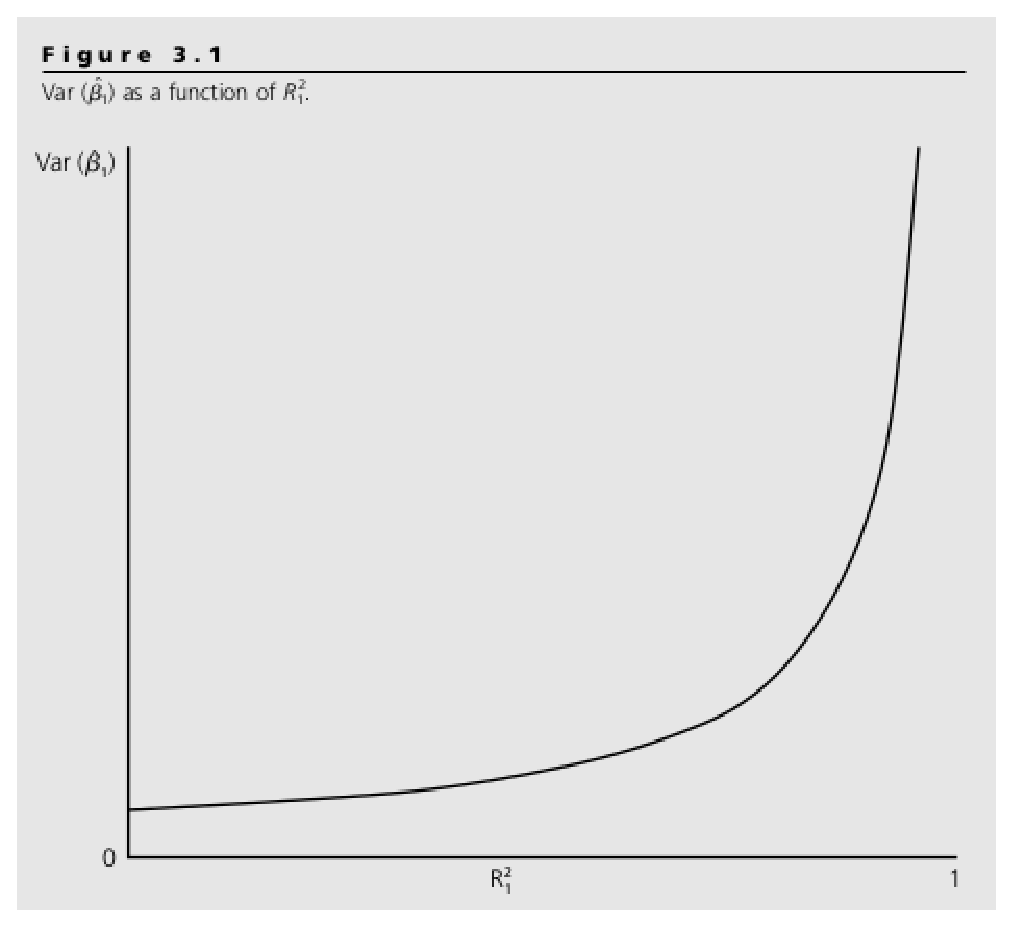
\includegraphics[scale = 0.5]{pictures/figure_3_1.eps}
\caption{$var[\hat{\beta}_j]$ jako funkce $R^2_j$}
\label{figure_3_1}
\end{figure} 

\subsection{Rozptyl v chybně specifikovaném regresním modelu}

Předpokládejme, že správně definovaný regresní model má podobu
\begin{equation}
y = \beta_0 + \beta_1 x_1 + \beta_2 x_2 + u.
\end{equation}
Dále předpokládejme, že namísto
\begin{equation}
\hat{y} = \hat{\beta}_0 + \hat{\beta}_1 x_1 + \hat{\beta}_2 x_2
\end{equation}
jsme odhadli model ve tvaru
\begin{equation}
\tilde{y} = \tilde{\beta}_0 + \tilde{\beta}_1 x_1.
\end{equation}
V takovém případě je $\tilde{\beta}_1$ zkreslené s výjimkou situace, kdy jsou $x_1$ a $x_2$ nekorelované. Pokud je zkreslení naším jediným 
kritériem výběru, pak preferujeme $\hat{\beta_1}$ před $\tilde{\beta}_1$. Pokud je však naším kritériem rozptyl odhadovaného parametru, pak 
můžeme naopak preferovat $\tilde{\beta}_1$ před $\hat{\beta_1}$, protože kromě situace, kdy $x_1$ a $x_2$ jsou nekorelované, je
\begin{equation}
var[\hat{\beta_1}] = \frac{\sigma^2}{SST_1(1 - R^2_1)}
\end{equation}
vždy větší než
\begin{equation}
var[\tilde{\beta}_1] = \frac{\sigma^2}{SST_1}.
\end{equation}
Proto bychom při rozhodování se mezi $\hat{\beta}_1$ a $\tilde{\beta}_1$ měli vzít v úvahu nejen velikost zkreslení, ale také velikost 
směrodatné odchylky odhadu. Je důležité si uvědomit, že směrodatná odchylka odhadu je také poplatná velikosti náhodného výběru. 
Další tak trochu skrytou skutečností je, že opominutím $x_2$ v regresním modelu se přesune část variability $x_2$ do 
rozptylu chyby $u$. Ta však není v rámci $var[\tilde{\beta}_1]$ zohledněna. Nižší variabilita $\tilde{\beta}_1$ tak může být poněkud zavádějící.

\subsection{Odhad $\sigma^2$}

OLS rezidua z odhadnutého modelu jsou definována jako
\begin{equation}
\hat{u}_i = y_i - \hat{\beta}_0 - \hat{\beta}_1 x_{i1} - \hat{\beta}_2 x_{i2} - ... - \hat{\beta}_k x_{ik}.
\end{equation}
Nezkreslený odhad jejich rozptylu $\sigma^2$ je pak roven
\begin{equation}
\hat{\sigma}^2 = \frac{\sum_{i = 1}^n \hat{u}_i^2}{n - k - 1} = \frac{SSR}{n - k - 1}.
\end{equation}
Člen $n - k - 1$ představuje počet stupňů volnosti obecného regresního modelu s $k$ vysvětlujícími veličinami odhadnutého nad náhodným 
výběrem o $n$ pozorováních. To, že úprava o počet stupňů volnosti je nezbytná, je zřejmé z podmínek prvního řádu 
pro OLS odhady. Tyto podmínky lze vyjádřit ve tvaru $\sum_{i = 2}^n \hat{u}_1 = 0$ a $\sum_{i = 1}^n x_{ij}\hat{u}_j = 0$, kde $j = 1, 2, ..., k$. Při 
odvození OLS odhadů je tak třeba aplikovat těchto $k+1$ omezení. To znamená, že pro daných $n - (k + 1)$ reziduí lze zbývajících $k + 1$ 
reziduí dopočíst na základě výše uvedených $k + 1$ omezení. Proto mají rezidua pouze $n - (k + 1)$ stupňů volnosti.
\begin{theorem}[Nestrannost odhadu $\sigma^2$]
Pokud jsou splněny Gauss-Markovy předpoklady MLR.1 až MLR.5, pak platí $E[\hat{\sigma}^2] = \sigma^2$.

\raggedleft{$\clubsuit$}
\end{theorem}
Směrodatná odchylka $\hat{\beta}_j$ je definována jako
\begin{equation}
sd(\hat{\beta}_j) = \frac{\sigma}{\sqrt{SST_j(1 - R^2_j)}}.
\end{equation}
Pokud $\sigma$ nahradíme jejím odhadem $\hat{\sigma}$, získáme tzv. směrodatnou chybu
\begin{equation}
se(\hat{\beta}_j) = \frac{\hat{\sigma}}{\sqrt{SST_j(1 - R^2_j)}}.
\end{equation}
Protože $se(\hat{\beta}_j)$ závisí na $\hat{\sigma}$, jedná se o náhodnou veličinu. Rovnice (3.43) není validním odhadem $sd(\hat{\beta}_j)$, 
pokud chyba $u$ vykazuje heteroskedasticitu.

\section{Efektivita OLS odhadu - Gauss-Markovova věta}

Při splnění předpokladů MLR.1 až MLR.5 jsou OLS odhady regresních parametrů nezkreslené. Při splnění těchto podmínek však kromě OLS odhadu existuje celá 
řada jiných nezkreslených lineárních odhadů. Nicméně OLS odhad je nejen nezkreslený, ale také efektivní, tj. má z těchto odhadů 
nejmenší rozptyl. Takovýto odhad nazýváme nejlepším nezkresleným lineárním odhadem (best linear unbiased estimator - BLUE).
\begin{theorem}[Gauss-Markovova věta]
Pokud jsou splněny Gauss-Markovovy předpoklady MLR.1 až MLR.5, pak platí $E[\hat{\sigma}^2] = \sigma^2$.

\raggedleft{$\clubsuit$}
\end{theorem}

Je třeba zdůraznit, že v případě heteroskedasticity je OLS 
odhad parametrů regresního modelu stále nezkreslený, nicméně již nemá nejmenší rozptyl mezi všemi možnými nezkreslenými lineárními odhady.
